\documentclass{article}
% packages
%% font, back-end
\usepackage[english]{babel} % more, non-english characters
\usepackage{csquotes} % back-end quotation forming
\usepackage[T1]{fontenc} % back-end for non-english characters
\usepackage{graphicx} % advanced graphics support

%% formatting
\usepackage{comment} % adds the comment environment
\usepackage[letterpaper,top=2.54cm,bottom=2.54cm,left=2.54cm,right=2.54cm,marginparwidth=1.75cm]{geometry} % page dimensions
\usepackage[colorlinks=true, allcolors=blue]{hyperref} % makes hyper-links
\usepackage{ragged2e} % text alignment
\usepackage{setspace} % linespacing
\doublespacing

%% math, symbols
\usepackage{amsmath} % math formulas
\usepackage{array} % arrays inside math mode
\usepackage{gensymb} % more symbols

%% figures, tables
\usepackage{booktabs} % better tables
\usepackage{longtable} % make tables that span multiple pages
\usepackage{multirow} % multi-columns and rows for tables
\usepackage{subfig} % allows for subfigures

%% bibliography, glossary
\usepackage[style=numeric, sorting=none, giveninits]{biblatex} % bibliography
\addbibresource{refs.bib}
\usepackage[acronym,nomain,nonumberlist,nogroupskip,nopostdot]{glossaries} % makes a glossary
\loadglsentries{glossary}
\newglossarystyle{mystyle}{%
  \glossarystyle{long}%
  \renewenvironment{theglossary}%
     {\begin{longtable}{p{2.5cm}p{\linewidth}}}%
     {\end{longtable}}%
}
\makeglossaries

% beginning of the document
\begin{document}
\begin{titlepage}

\centering
\scshape
\vspace{\baselineskip}

\rule{\textwidth}{1.6pt}\vspace*{-\baselineskip}\vspace*{2pt}
\rule{\textwidth}{0.4pt}

{\Huge \textbf{\textsc{NPRE 458: Group 4 \\ TEMPLATE \\ \vspace{15pt}}}}

\rule{\textwidth}{0.4pt}\vspace*{-\baselineskip}\vspace{3.2pt}
\rule{\textwidth}{1.6pt}\vspace{6pt}
\centerline{\textit{University of Illinois at Urbana-Champaign}} \\
\centerline{\textit{Department of Nuclear, Plasma, and Radiological Engineering}}
\vspace{1.5\baselineskip}

\large \centerline{\textbf{Members}}

\large \centerline{David Barnett}
\small \centerline{davidbb2}

\large \centerline{Nathan Glaser}
\small \centerline{nglaser3}

\large \centerline{Joseph Specht}
\small \centerline{jspecht3}

\vspace{2\baselineskip}

\large \centerline{{\bf Professor}}
\large \centerline{James Stubbins}
\quad

\vfill
\large \centerline{MONTH DAY, 2025}
%
\pagenumbering{gobble}
\end{titlepage}

\tableofcontents
\clearpage
\pagenumbering{arabic}

\printglossary
\clearpage

\section{Glossary}
To use the glossary package, type \gls{nrc}. The first time an acronym is used, it will spell the acronym out and give the abbreviation. After the first time, only the abbreviation will be used \gls{nrc}. You can also make the entries plural with \glspl{msr}. These glossary entries need to be added into glossary.tex.


\section{Spacing}
You can clear a page with \textbackslash clearpage. You can set spacing with \textbackslash vspace\{XXXcm\} or vspace\{XXXpt\} or vspace\{XXX\textbackslash baselineskip\}. Respectively, each vspace makes a gap in centimeters, font size points, and the number of lines between the line above and below the command.


\section{Figures}
You can type \textbackslash begin\{figure\} and hit tab to get an auto-populated figure with automatic centering. Put and [!h] after begin\{figure\} to get the picture to insert in between this paragraph and the next. This [!h] can be finicky, so it might take some finagling. An example of a figure is given below.

\begin{figure}[!h]
    \centering
    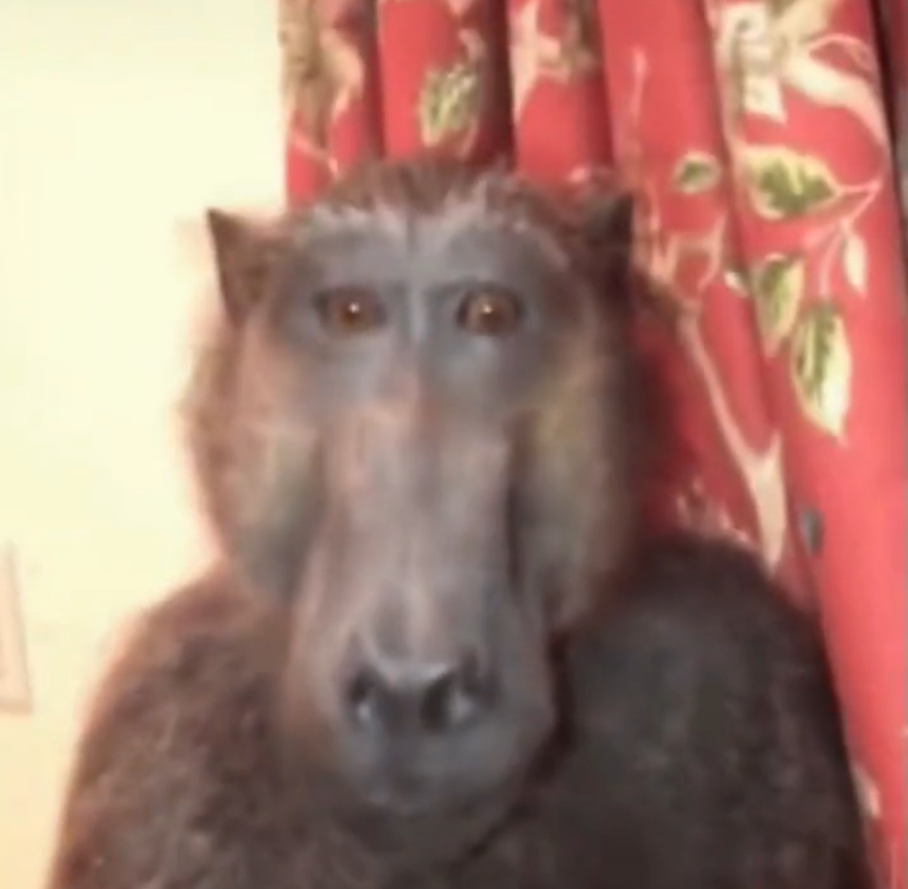
\includegraphics[width=0.5\linewidth]{pictures/example-picture.png}
    \caption{Figure Example.}
    \label{fig:example-figure}
\end{figure}

\clearpage
\subsection{Sub-Figures}
You can also make sub-figures. You can separate each figure with \textbackslash quad, short for four spaces, and put the figures on a new line with \textbackslash\textbackslash. You may need to change the width of the figure from the default of 0.5 of the line width to get the figures to fit. An example is given below.

\begin{figure}[!h]
    \centering
    \subfloat[\centering Title 1]{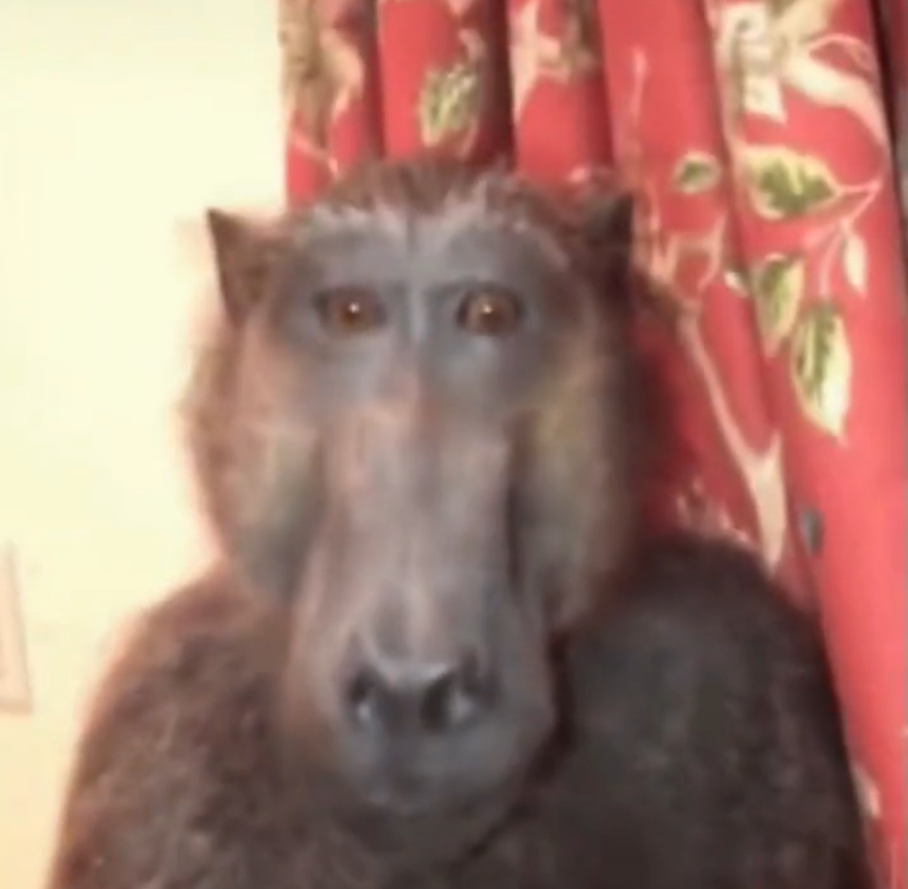
\includegraphics[width=0.4\linewidth]{pictures/example-picture.png}} \quad 
    \subfloat[\centering Title 2]{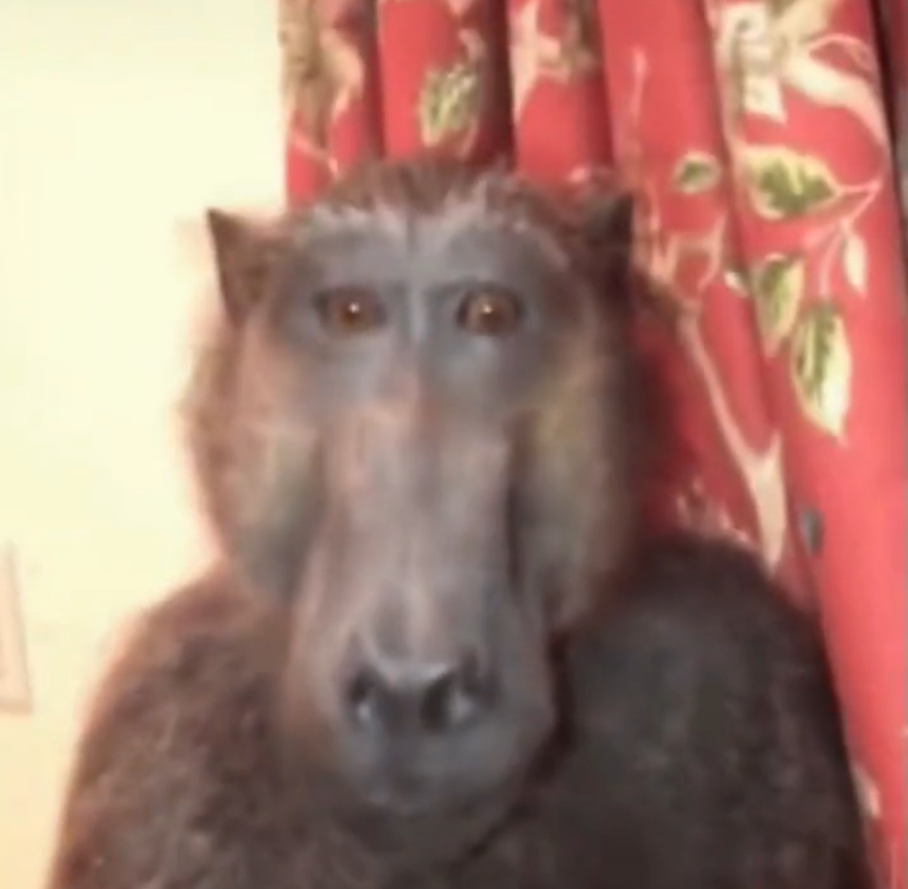
\includegraphics[width=0.4\linewidth]{pictures/example-picture.png}} \\
    \subfloat[\centering Title 3]{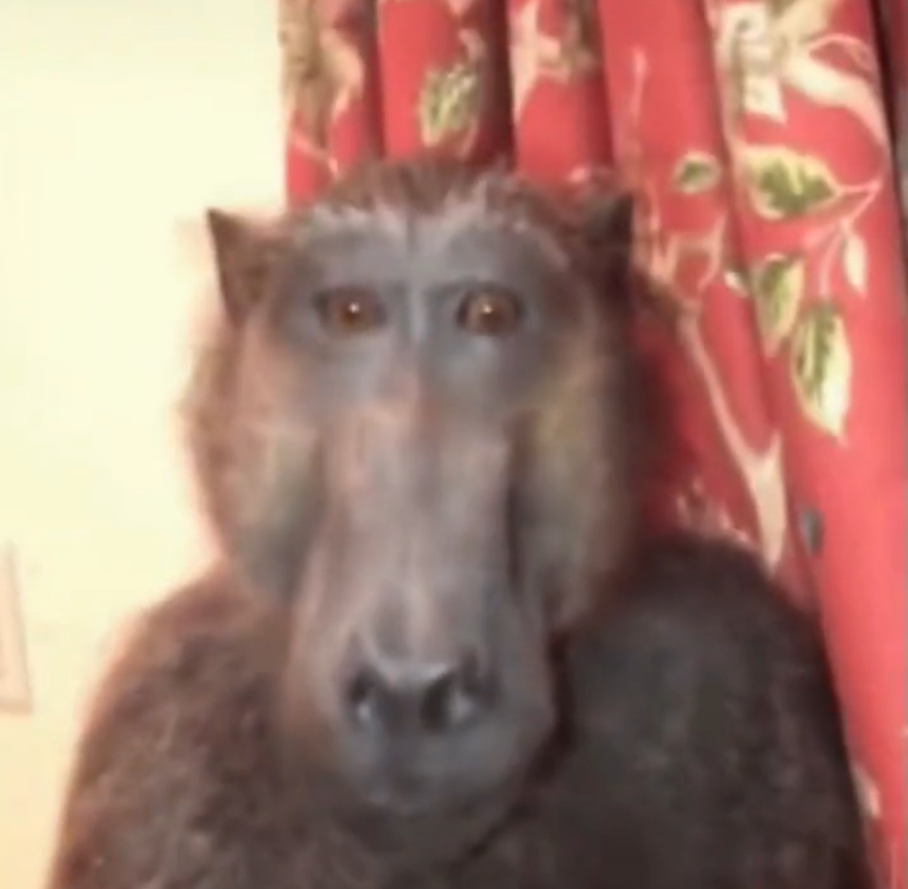
\includegraphics[width=0.4\linewidth]{pictures/example-picture.png}}
    \quad
    \subfloat[\centering Title 4]{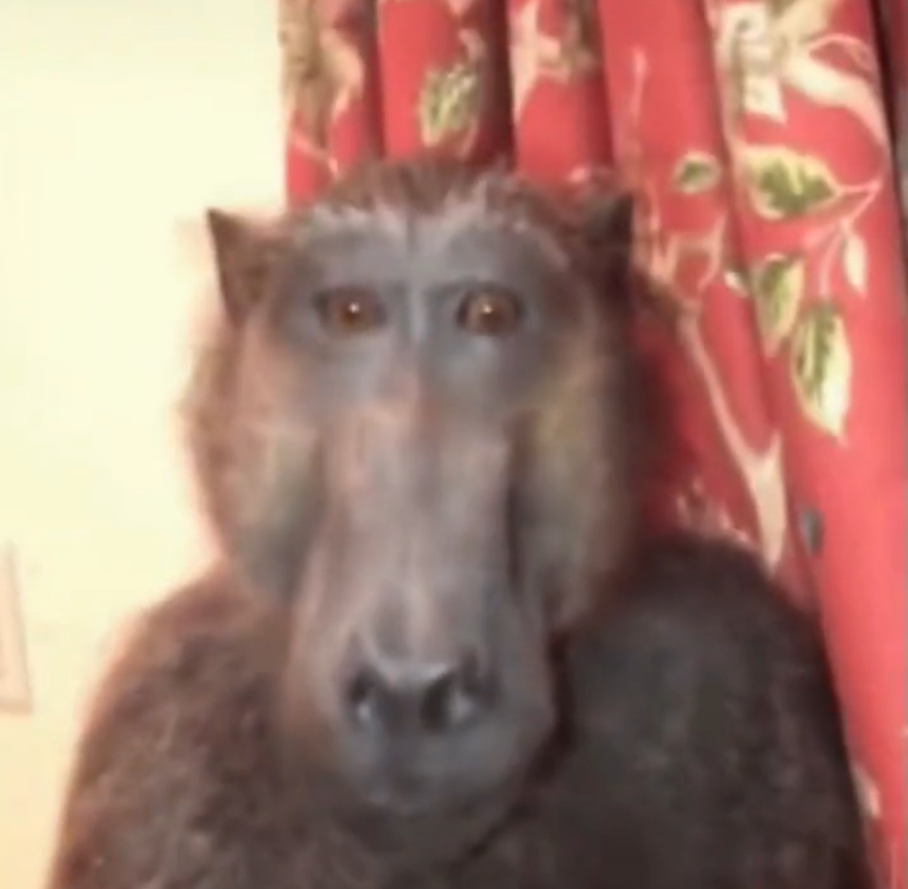
\includegraphics[width=0.4\linewidth]{pictures/example-picture.png}}
    \caption{Sub-Figure Example.}
    \label{fig:subfigure-example}
\end{figure}


\clearpage
\section{Sub-Sections}
Here would be the information pertaining to everything in this section.

\subsection{Sub-Section}
This is how you get a sub-section.

\subsubsection{Sub-Sub-Section}
This is a sub-sub-section. There are no sub-sub-sub sections.


\section{Tables}
Tables can be made with \textbackslash begin\{table\} and hitting tab. The default table has the caption at the bottom of the table, so move it below the \textbackslash centering line. Also, the default table is single-spaced, so add \textbackslash def \textbackslash arraystretch{1.5} below centering.

You can add columns in the section that has \{c|c\} by adding more c's. This example array has 5 columns, so |c|c|ccc|. The lines between the c's mean a vertical line between each column. For lines between each row, use either \textbackslash hline to span the entire table or \textbackslash cline\{x-y\} to span from column x to y.

This table shows how to make multi-row and multi-column blocks in the table. This example is fairly dense, however, the table reads from left-to-right then top-to-bottom.

\begin{table}[!h]
    \centering
    \def\arraystretch{1.5}
    \caption{Example Table.}
    \begin{tabular}{|c|c|ccc|} \hline
        \multicolumn{2}{|c|}{\multirow{2}{*}{\bf Big Block}} & \multicolumn{3}{|c|}{\bf Multiple Columns} \\ \cline{3-5}
        
        \multicolumn{2}{|c|}{\multirow{2}{*}{ \ }} & {\bf Sub-Heading 1} & {\bf Sub-Heading 2} & {\bf Sub-Heading 3} \\ \hline
        
        \multirow{2}{*}{\bf Multi-Row} & {\bf MRS-1} & - & - & - \\ \cline{3-5}
        
        \ & {\bf MRS-2} & - & - & - \\ \hline
    \end{tabular}
    \label{tab:example-table}
\end{table}


\clearpage
\section{Math}
You can create an equation with \textbackslash begin\{equation\}. In equation mode, you can type type a \textbackslash \ then the name of the symbol you want. You can also label equations with \textbackslash label\{\} for future reference.

\begin{equation}
    \label{eq:example-eq}
    \eta = \zeta
\end{equation}

\subsection{subequations}
If you have multiple equations that go together or are steps in the same derivation, you can use sub-equations to group them together. You can label sub-equations like equations.
\begin{subequations}
    \label{eq:example-subeq}
    \begin{equation}
        \frac{\alpha}{\beta} = B^{super}_{sub}
    \end{equation}
    \begin{equation}
        \sqrt{\gamma} = \delta \cdot \Delta = \delta \Delta
    \end{equation}
    \begin{equation}
        \omega \neq \epsilon \leq \Xi \geq \chi
    \end{equation}
\end{subequations}

\section{Referencing}
You can reference previous figures, equations, and tables with \textbackslash ref\{\}. To cite figures and sub-figures, use Fig. \ref{fig:example-figure}. To cite tables, use Table \ref{tab:example-table}. To cite equations, use Eq. \ref{eq:example-eq}.

\clearpage
\section{Lists}
You can make lists with \textbackslash begin\{enumerate \} for numbered lists or \textbackslash begin\{itemize \} for regular lists. A list inside another list makes a sub-list.

Here is an enumerate:
\begin{enumerate}
    \item item 1
    \begin{enumerate}
        \item sub-item 1
        \item sub-item 2
        \item sub-item 3
    \end{enumerate}
    \item Item 2
    \begin{enumerate}
        \item sub-item 1
        \begin{enumerate}
            \item sub-sub-item 1
            \begin{enumerate}
                \item sub-sub-sub-item 1
                \item this is as deep as you can nest
            \end{enumerate}
        \end{enumerate}
    \end{enumerate}
\end{enumerate}

And here is an itemize:
\begin{itemize}
    \item item 1
    \item item 2
    \item item 3
    \item item 4
\end{itemize}


\clearpage
\section{Citations}
To have citations, add something to the refs.bib and then you can cite it like this \cite{example-citation}. You can add sources to cite by adding them in refs.bib.

\printbibliography
\end{document}
